\chapter{Transmisión OFDM en Estándar IEEE 802.11a}
\label{Ch:2}
\graphicspath{{figs/}}

En la sección 17.3 del estándar IEEE 802.11\cite{ieee} se definen las especificaciones a nivel físico de la transmisión por señales OFDM. El estándar define las técnicas utilizadas para traducir los datos provenientes de capas superiores a formas de ondas que se transmitirán por el medio inalámbrico utilizando OFDM, así como los métodos utilizados para asegurar que el receptor sea capaz de reconocer e interpretar las señales transmitidas.

En este capítulo se resumen los aspectos del estándar IEEE 802.11 relevantes para el desarrollo del proyecto, partiendo de la descripción de la unidad fundamental de la señal, el símbolo OFDM.

Una vez definido el símbolo OFDM, se procede a describir la estructura del mensaje que se transmitirá por el medio inalámbrico, que recibe el nombre de PPDU por sus siglas en inglés.

Finalmente se detalla la primer parte de la PPDU, llamada preámbulo. El preámbulo cumple la función de facilitar la detección y el sincronismo de la señal en el receptor, por lo que es de especial importancia para este proyecto.

\section{Símbolo OFDM}
\label{S:ch2-simbolo}

El símbolo OFDM es la unidad fundamental transmitida en OFDM. La construcción del mismo se basa en especificaciones tanto en el dominio de la frecuencia como en el dominio del tiempo.

Un símbolo OFDM es una descripción de 48 números complejos resultantes de determinada constelación de modulación (el estándar admite BPSK, QPSK, 16-QAM, o 64-QAM) que describen las componentes en frecuencia de una forma de onda. 

Las componentes en frecuencia se transforman al dominio del tiempo en una ventana temporal de duración definida por el estándar. 

\subsection{Duración Temporal del Símbolo}
\label{Ss:ch2-tiempo-simbolo}

El estándar define, en función del espacio entre subportadoras, varios tiempos de interés. En particular, los parámetros de interés se describen en la tabla \ref{tab:tiempos-formula}, así como las fórmulas usadas para calcularlos en función de los demás parámetros.\\
\begin{table}[ht]
    \centering{}
    \begin{tabular}{|l|l|l|}
    \hline
     \thead{Parámetro} & \thead{Significado} & \thead{Fórmula}\\
     \hline
     $T_{FFT}$ & Duración de los intervalos de IFFT y FFT. & $1/\Delta_F$  \\
     $T_{GI}$  & Intervalo de guarda para los símbolos OFDM. & $T_{FFT}/4$      \\
     $T_{SYM}$ & Duración de un símbolo OFDM. & $T_{GI}+T_{FFT}$ \\
     $T_{GI2}$ & Intervalo de guarda para los campos del preámbulo. & $T_{FFT}/2$      \\
     $T_{SHORT}$ & Duración de la primer secuencia de entrenamiento. & $10\times T_{FFT}/4$  \\
     $T_{LONG}$ & Duración de la segunda secuencia de entrenamiento. & $T_{GI2}+2\times T_{FFT}$ \\
     \hline
    \end{tabular}
    \caption{Tabla de parámetros temporales y sus fórmulas en función del parámetro $\Delta_F$, el espaciamiento entre subportadoras.\label{tab:tiempos-formula}}
\end{table}

El parámetro del cual surgen los otros, el espacio entre subportadoras $\Delta_F$, depende del espaciamiento entre los canales en el dominio de la frecuencia. El espaciamiento entre subportadoras es una 64-ava parte del espaciamiento entre canales.

En el funcionamiento típico, los canales están espaciados 20 MHz, pero el sistema admite operación en modo \textit{half-clocked}, con espaciamiento de 10 MHz, y \textit{quarter-clocked}, con espaciamiento de 5 MHz. Los valores de los parámetros temporales en función del espaciamiento entre canales se resumen en la tabla \ref{tab:tiempos-valor}.\\
\begin{table}[ht]
    \centering{}
    \begin{tabular}{|l|c|c|c|}
    \hline
     \thead{Parámetro} & \thead{Valor con canales\\espaciados 20 MHz}& \thead{Valor con canales\\espaciados 10 MHz} & \thead{Valor con canales\\espaciados 5 MHz} \\
     \hline
     $T_{FFT}$   & $3.2$ \textmu s & $6.4$ \textmu s & $12.8$ \textmu s \\
     $T_{GI}$    & $0.8$ \textmu s & $1.6$ \textmu s & $3.2$ \textmu s \\
     $T_{GI2}$   & $1.6$ \textmu s & $3.2$ \textmu s & $6.4$ \textmu s \\
     $T_{SYM}$   & $4$ \textmu s & $8$ \textmu s & $16$ \textmu s \\
     $T_{SHORT}$ & $8$ \textmu s & $16$ \textmu s & $32$ \textmu s \\
     $T_{LONG}$  & $8$ \textmu s & $16$ \textmu s & $32$ \textmu s \\
     \hline
    \end{tabular}
    \caption{Tabla de valores temporales según el espaciamiento entre canales admitidos por el estándar IEEE 802.11.\label{tab:tiempos-valor}}
\end{table}

La importancia del parámetro $T_{FFT}$ se describe en mayor detalle en la sección \ref{Ss:ch2-ifft}, y su relación con los parámetros $T_{GI}$ y $T_{SYM}$ se detalla en la sección \ref{Ss:ch2-prefijo}. A su vez, los parámetros $T_{GI2}$, $T_{SHORT}$ y $T_{LONG}$ hacen referencia al preámbulo y se detallan en la sección \ref{S:ch2-preambulo}.

\subsection{Definición de Subportadoras}
\label{Ss:ch2-subportadoras}

Este símbolo está compuesto por un total de 52 subportadoras, de las cuales 48 transportan datos y las 4 restantes transportan ondas piloto. Para la asignación de portadoras, se toman 48 números resultantes de la etapa de modulación, enumerados de 0 a 47, las subportadoras se enumeran de -26 a 26 y se asignan de la siguiente forma.\\
\begin{figure}[ht]
    \centering{}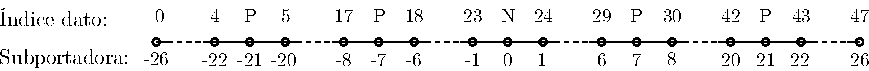
\includegraphics[width=\imsizeL]{asignacion_subportadoras.pdf}
    \caption{Asignación de números según sus índices a subportadoras que constituyen un símbolo OFDM.\label{fig:asignacion-subportadoras}}  
\end{figure}

Las ondas piloto, representadas con la letra P en la figura \ref{fig:asignacion-subportadoras}, son asignadas a las subportadoras en índices -21, -7, 7, y 21. Tienen el propósito de preservar el sincronismo durante la transmisión, con métodos que exceden el alcance de este proyecto. La subportadora de índice 0, a su vez, siempre mantiene un valor nulo. 

\subsection{IFFT}
\label{Ss:ch2-ifft}
Las subportadoras con sus correspondientes valores asignados son una representación en el dominio de la frecuencia del símbolo OFDM. Esta representación se transforma al dominio del tiempo con un módulo IFFT. Típicamente se utilizan módulos IFFT con un número de puntos potencia de 2 (mínimamente 64) y para obtener una correcta transformación del dominio se aplica una operación de desplazamiento, transportando las subportadoras de índice negativo al final del vector a transformar.\\
\begin{figure}[ht]
    \centering{}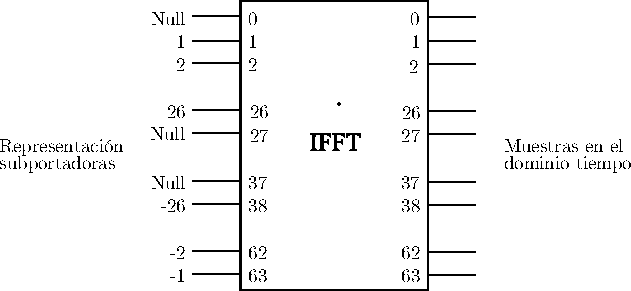
\includegraphics[width=\imsize]{IFFT.pdf}
    \caption{Esquema de aplicación de IFFT de 64 puntos a una descripción en subportadoras de un símbolo OFDM.\label{fig:ifft64}}  
\end{figure}

En el estándar se define la transformación con una IFFT de 64 puntos, sin embargo, aplicando el mismo desplazamiento sobre una IFFT de un número mayor de puntos es posible y se obtiene la misma señal con mayor resolución temporal.\\
\begin{figure}[ht]
    \centering{}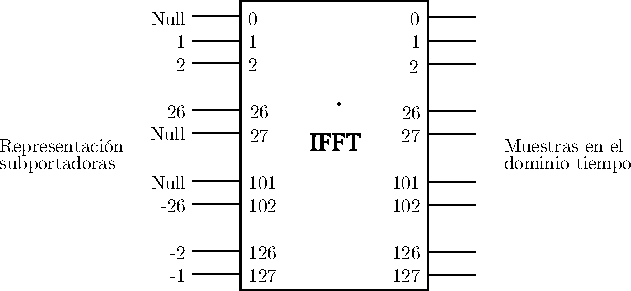
\includegraphics[width=\imsize]{IFFT128.pdf}
    \caption{Esquema de aplicación de IFFT de 128 puntos a una descripción en subportadoras de un símbolo OFDM.\label{fig:ifft128}}  
\end{figure}

Independientemente del número de puntos utilizados en la IFFT, la duración de la representación en el dominio temporal resultante ocupa el tiempo $T_{FFT}$ definido en la tabla \ref{tab:tiempos-valor}.

\subsection{Prefijo Cíclico}
\label{Ss:ch2-prefijo}

Aplicada la IFFT, al vector resultante se le agrega en intervalo de guarda, $GI$, el cual tiene la función de mitigar efectos de interferencia inter-símbolos (ISI por sus siglas en inglés), este fenómeno se detalla en el capítulo \ref{Ch:3}. El GI consiste en un prefijo cíclico de la señal temporal, y se construye de la siguiente forma.

\begin{enumerate}
    \item De las $N_{FFT}$ muestras salientes de la operación IFFT, se toman las últimas $N_{FFT}/4$ muestras. 
    \item Las últimas $N_{FFT}/4$ muestras se copian y se concatenan al inicio de las muestras existentes, y reciben el nombre de prefijo cíclico. 
    \item La concatenación del prefijo cíclico con las muestras existentes es el símbolo OFDM que se transmitirá.
\end{enumerate}

El procedimiento se representa gráficamente en la figura \ref{fig:prefijo}.\\
\begin{figure}[ht]
    \centering{}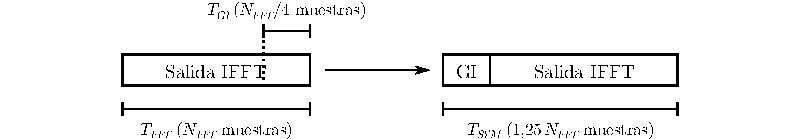
\includegraphics[width=\imsize]{prefix.pdf}
    \caption{Diagrama de aplicación de intervalo de guarda (prefijo cíclico) a un símbolo OFDM.\label{fig:prefijo}}  
\end{figure}


\section{Estructura de la PPDU}
\label{S:ch2-ppdu}

La PPDU consiste en una secuencia de símbolos OFDM que transmiten un mensaje a través de la capa física, descripta en la Figura \ref*{fig:ppdu}. Incorpora al mensaje la información requerida para detección, sincronismo, demodulación, y decodificación del mismo.\\
\begin{figure}[ht]
    \centering{}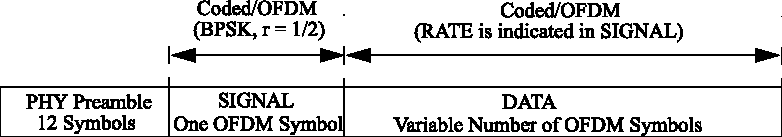
\includegraphics[width=\imsize]{PPDU.pdf}
    \caption{Estructura de alto nivel de una PPDU según es definida en el estándar IEEE 802.11.\cite{ieee}\label{fig:ppdu}}  
\end{figure}

Los campos que la constituyen son los siguientes
\begin{enumerate}
    \item PHY Preamble: Secuencia de símbolos predeterminados utilizados para detección, sincronismo, y estimación del canal.
    \item SIGNAL: Símbolo OFDM que transmite la información necesaria para la recepción de DATA a través de los campos LENGTH y RATE. Siempre es modulado en BPSK y codificado a tasa 1/2.
    \item DATA: Número variable de símbolos que transmiten el \textit{payload} del mensaje, el número de símbolos es informado por LENGTH, y la modulación y tasa de código utilizadas son determinadas únivocamente por RATE.
\end{enumerate}

Los campos SIGNAL y DATA exceden el alcance del proyecto, por lo que no se estudiarán en mayor detalle, pero el campo PHY Preamble es fundamental al proyecto. La forma en la que se construye se detalla en la sección siguiente.

\section{PHY Preamble}
\label{S:ch2-preambulo}

El preámbulo, la forma de onda predeterminada transmitida al inicio de cada PPDU, se construye de forma similar a otros símbolos, partiendo de definiciones predefinidas de las 52 subportadoras. Se definen dos símbolos en particular, el símbolo corto de entrenamiento y el símbolo largo de entrenamiento.

En la construcción de los símbolos de entrenamiento no existen ondas piloto, se fijan valores diréctamente a las 52 subportadoras previo a la etapa IFFT, con valores definidos por $S$ en el caso del símbolo corto y $L$ en el caso del símbolo largo.

Otra diferencia con la construcción de los símbolos normales reside en que estos símbolos de entrenamiento tienen el doble de duración, usando los valores $T_{SHORT}$ y $T_{LONG}$ registrados en la tabla \ref{tab:tiempos-valor}. La aplicación del prefijo cíclico es similar a la descrita en la sección \ref{Ss:ch2-prefijo}, con la diferencia de que el prefijo cíclico es el doble de longitud, y se transmiten 2 períodos de la señal resultante de la IFFT. El procedimiento se describe en la figura \ref{fig:training-symbol}.\\
\begin{figure}[ht]
    \centering{}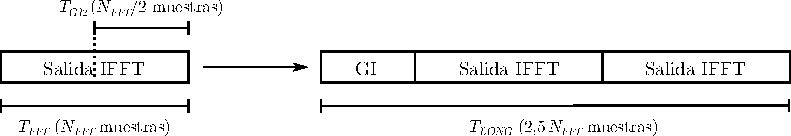
\includegraphics[width=\imsize]{training_symbol.pdf}
    \caption{Diagrama de aplicación de intervalo de guarda (prefijo cíclico) a una secuencia de entrenamiento del preámbulo.\label{fig:training-symbol}}  
\end{figure}


\subsection{Símbolo Corto de Entrenamiento}
\label{Ss:ch2-short}

El símbolo corto de entrenamiento se usa para construir la primer secuencia transmitida. La asignación de valores a subportadoras es definida por la ecuación \ref{eq:def-S}.\\
\begin{equation}\label{eq:def-S}
    \begin{aligned}
    S_{-26,26} = \sqrt{13/6}\, 
    [0 ,\,  0   ,\, 1+j ,\,  0   ,\, 0 ,\,  0   ,\, -1-j ,\,  0   ,\, 0 ,\, 0   ,\, 1+j ,\, 0   ,\, 0 ,\, 
     0 ,\, -1-j ,\, 0   ,\,  0   ,\, 0 ,\\ -1-j ,\,  0   ,\,  0   ,\, 0 ,\, 1+j ,\, 0   ,\, 0   ,\, 0 ,\, 0 ,\,
     0 ,\,  0   ,\, 0   ,\, -1-j ,\, 0 ,\,  0   ,\,  0   ,\, -1-j ,\\ 0 ,\, 0   ,\, 0   ,\, 1+j ,\, 0 ,\, 
     0 ,\,  0   ,\, 1+j ,\,  0   ,\, 0 ,\,  0   ,\,  1+j ,\,  0   ,\, 0 ,\, 0   ,\, 1+j ,\, 0   ,\, 0]
    \end{aligned}
\end{equation}
    
En particular, $S$ asigna valores complejos únicamente a subportadoras de índice múltiplo de 4. Esta asignación se representa gráficamente en la figura \ref{fig:short-sc}.\\
\begin{figure}[ht]
    \centering{}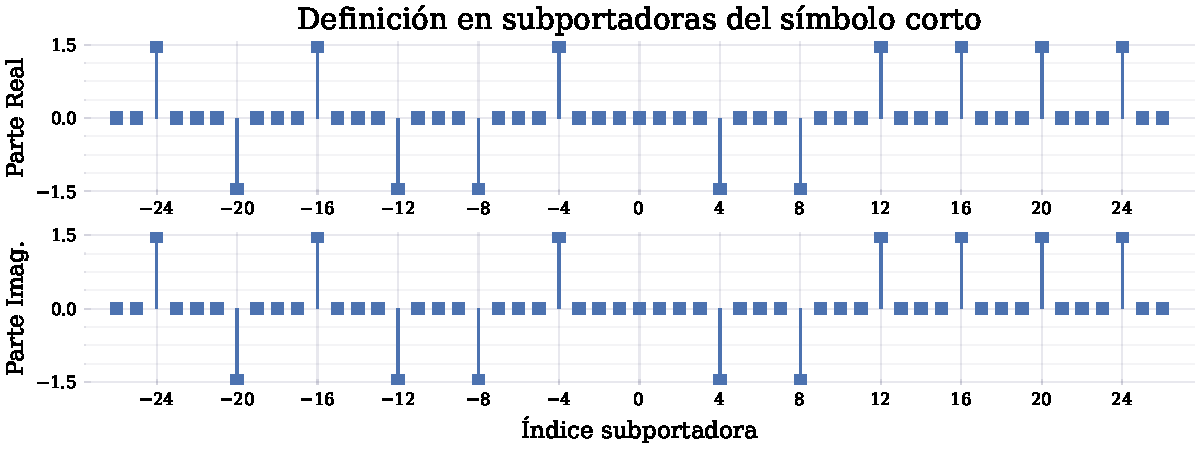
\includegraphics[width=\imsize]{short_sc.pdf}
    \caption{Asignación de subportadoras para la construcción del símbolo corto de entrenamiento.\label{fig:short-sc}}  
\end{figure}

Una aplicación de la IFFT a $S$ resulta en una señal periódica, de la cual 4 períodos entran en $T_{FFT}$. Aplicar el procedimiento descrito en la figura \ref{fig:training-symbol} se obtienen 10 períodos de la señal, la cual se grafica en la figura \ref{fig:short-time}.\\ 
\begin{figure}[ht]
    \centering{}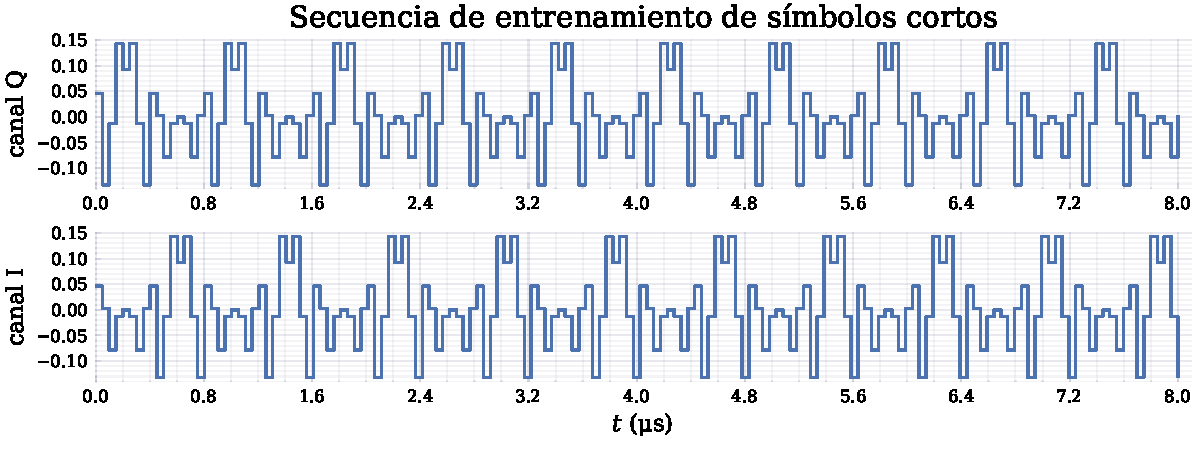
\includegraphics[width=\imsize]{short_time.pdf}
    \caption{Secuencia de entrenamiento de símbolos cortos en el dominio temporal.\label{fig:short-time}}  
\end{figure}

La señal vista en la figura \ref{fig:short-time} recibe nombre de \textit{secuencia de entrenamiento de símbolos cortos}. Esta secuencia cumple la función de facilitar la detección de la señal entrante en el receptor, así como permitir algoritmos preliminares de sincronismo, y es de vital importancia para este proyecto.


\subsection{Símbolo Largo de Entrenamiento}
\label{Ss:ch2-long}

El símbolo corto de entrenamiento se usa para construir la segunda secuencia transmitida. La asignación de valores a subportadoras es definida en la ecuación \ref{eq:def-L}.\\
\begin{equation}\label{eq:def-L}
    \begin{aligned}
    L = 
    [1,\, 1,\, -1,\, -1,\, 1,\, 1,\, -1,\, 1,\, -1,\, 1,\, 1,\, 1,\, 1,\, 1,\, 1,\, -1,\, -1,\\
    1,\, 1,\, -1,\, 1,\, -1,\, 1,\, 1,\, 1,\, 1,\, 
    0,\,
    1,\, -1,\, -1,\, 1,\, 1,\, -1,\, 1,\, -1,\, 1,
    \\ -1,\, -1,\, -1,\, -1,\, -1,\, 1,\, 1,\, -1,\, -1,\, 1,\, -1,\, 1,\, -1,\, 1,\, 1,\, 1,\, 1]
    \end{aligned}
\end{equation}
    
A diferencia del caso del símbolo corto, $L$ asigna valores a todas las subportadoras disponibles. Esta asignación se representa gráficamente en la figura \ref{fig:long-sc}.\\
\begin{figure}[ht]
    \centering{}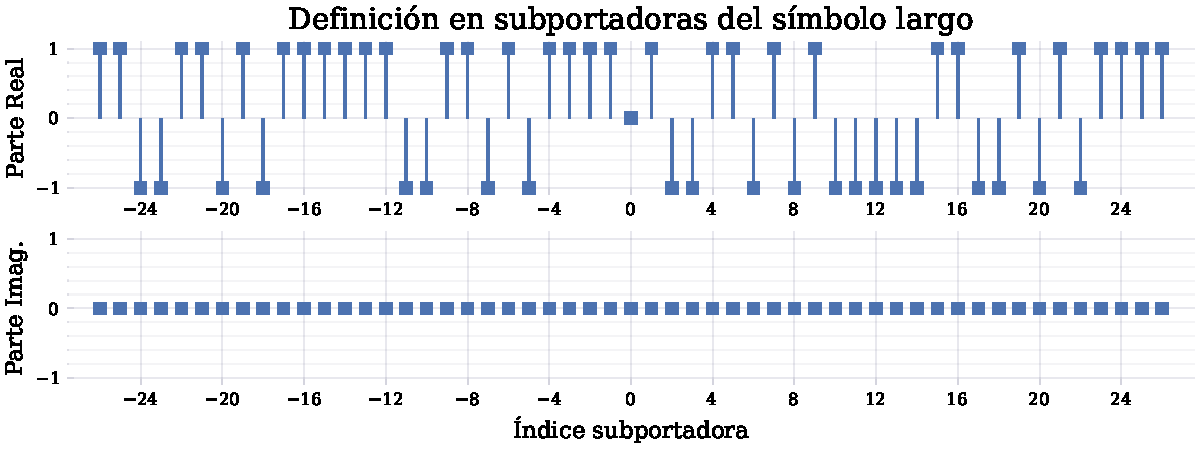
\includegraphics[width=\imsize]{long_sc.pdf}
    \caption{Asignación de subportadoras para la construcción del símbolo largo de entrenamiento.\label{fig:long-sc}}  
\end{figure}

Aplicar el procedimiento descrito en la figura \ref{fig:training-symbol} a $L$ resulta en la señal graficada en la figura \ref{fig:short-time}.\\ 
\begin{figure}[ht]
    \centering{}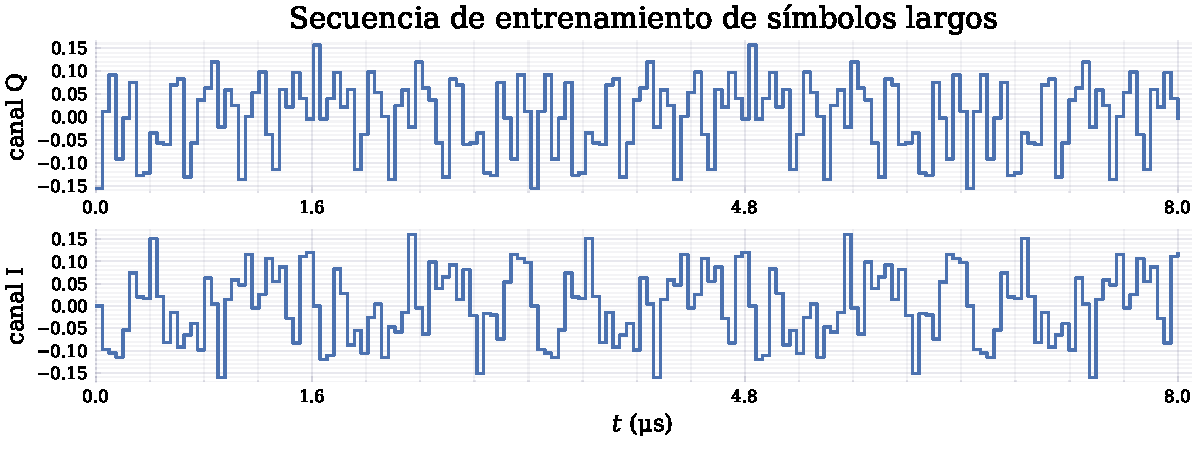
\includegraphics[width=\imsize]{long_time.pdf}
    \caption{Secuencia de entrenamiento de símbolos largos en el dominio temporal.\label{fig:long-time}}  
\end{figure}

Esta señal recibe el nombre de \textit{secuencia de entrenamiento de símbolos largos}. Sus funciones incluyen permitir algoritmos de sincronismo fino en el receptor, así como funciones de estimación del canal.

\section{Resumen del Capítulo}

En el capítulo se resumieron los aspectos de transmisión OFDM en el estándar IEEE 802.11 necesarios para poder llevar adelante el proyecto. Se entiende el procedimiento para construir un símbolo OFDM a partir de una secuencia de números resultantes de una constelación de modulación y como estos símbolos se organizan para formar una PPDU.

Se presta particular atención al campo PHY Preamble, específicamente a su primer mitad, la secuencia de de entrenamiento de símbolos cortos. Conociendo la forma y las propiedades de esta secuencia de entrenamiento se puede proceder a implementar algoritmos de detección y sincronismo en los capítulos siguientes.

%%% Local Variables: 
%%% mode: latex
%%% TeX-master: "template"
%%% End: 
